% created on 2022-03-24
% @author : c. kantana

\documentclass[a4paper, twoside, 12pt]{report}
\usepackage{geometry}
\geometry{top=1.5cm, bottom=2cm, left=2.5cm, right=2.5cm}
\usepackage{graphicx}
\usepackage{amsmath}
\usepackage{array}
\usepackage{subcaption}
\setcounter{secnumdepth}{5}
\setcounter{tocdepth}{2}
\usepackage{multirow}
\usepackage{adjustbox}
\usepackage{lmodern} 
\usepackage[]{algorithm2e}
\RestyleAlgo{boxruled}
\usepackage{amssymb}
\usepackage{rotating}
\usepackage{xcolor}

\usepackage{pdfpages}

\usepackage{hyperref}
\hypersetup{
	colorlinks=true,
	linkcolor=black,
	urlcolor=blue,
	citecolor=blue,
	linktoc=all
}

\definecolor{UnivBlue}{RGB}{47, 42, 133}
 

\begin{document}
	
	\newpage
	
	\AddToShipoutPictureBG*
	{
		
\includegraphics[width=\paperwidth,height=\paperheight]{Logo/background.jpg}
	}
	
	\begin{figure}[!h]
		\centering
		 \vspace{1.02cm}\hspace{-9cm}
\includegraphics[width=0.5\textwidth]{Logo/logoGE.png}
	\end{figure}

	\vspace{0.5cm}

	\hspace{-0.6cm}{\LARGE \textcolor{UnivBlue}{\textbf{Titre de la thèse}}}\\
	
	\large
	
	\hspace{-0.6cm}\textbf{Thèse de doctorat de l'Université Gustave Eiffel}\\

	\normalsize
	\hspace{-0.6cm}{École doctorale n° d’accréditation, dénomination et sigle}\\
	\hspace{-0.6cm}{Spécialité de doctorat: voir annexe}\\
	\footnotesize	
	\hspace{-0.6cm}{Unité de recherche : voir annexe }\\
	
	\large
	
	\hspace{-0.6cm}\textbf{Thèse présentée et soutenue à l’Université Gustave Eiffel,}\\
	\hspace{-0.6cm}\textbf{le 10/12/2021, par : }\\
	
	\vspace{0.3cm}
	
	\LARGE
	\hspace{-0.6cm}{\LARGE \textcolor{UnivBlue}{\textsc{\textbf{Prénom NOM}}}}\\
	
	\large
	
	\hspace{2cm} \textbf{Composition du Jury}
	
	\begin{table}[!h]
		\small
		\begin{tabular}{l l}
			\hspace{2.6cm}\textbf{Prénom NOM} & \multirow{2}{*}{\footnotesize \hspace{2cm} Président (e) du jury}\\
			\hspace{2.6cm}\footnotesize Titre, Affiliation & \\
			\hspace{2.6cm}\textbf{Prénom NOM} & \multirow{2}{*}{\footnotesize \hspace{2cm} Examinatrice}\\
			\hspace{2.6cm}\footnotesize Titre, Affiliation & \\
			\hspace{2.6cm}\textbf{Prénom NOM} & \hspace{2cm}\multirow{2}{*}{\footnotesize \hspace{-0cm} Examinateur}\\
			\hspace{2.6cm}\footnotesize Titre, Affiliation & \\
			\hspace{2.6cm}\textbf{Prénom NOM} & \hspace{2cm}\multirow{2}{*}{\footnotesize \hspace{-0cm} Rapportrice}\\
			\hspace{2.6cm}\footnotesize Titre, Affiliation & \\
			\hspace{2.6cm}\textbf{Prénom NOM} & \hspace{2cm}\multirow{2}{*}{\footnotesize \hspace{-0cm} Rapporteur}\\
			\hspace{2.6cm}\footnotesize Titre, Affiliation & \\
			\hspace{2.6cm}\textbf{Prénom NOM} & \hspace{2cm}\multirow{2}{*}{\footnotesize \hspace{-0cm} Invité}\\
			\hspace{2.6cm}\footnotesize Titre, Affiliation & \\
		\end{tabular}
	\end{table}	

	\large
	
	\hspace{2cm} \textbf{Encadrement de la thèse}

	\begin{table}[!h]
		\small
		\begin{tabular}{l l}
			\hspace{2.6cm}\textbf{Prénom NOM} & \hspace{2cm}\multirow{2}{*}{\footnotesize \hspace{-0cm} Directeur de thèse}\\
			\hspace{2.6cm}\footnotesize Titre, Affiliation & \\
			\hspace{2.6cm}\textbf{Prénom NOM} & \hspace{2cm}\multirow{2}{*}{\footnotesize \hspace{-0cm} Co-Directrice de thèse}\\
			\hspace{2.6cm}\footnotesize Titre, Affiliation & \\
			\hspace{2.6cm}\textbf{Prénom NOM} & \hspace{2cm}\multirow{2}{*}{\footnotesize \hspace{-0cm} Co-Encadrant de thèse}\\
			\hspace{2.6cm}\footnotesize Titre, Affiliation & \\
			\hspace{2.6cm}\textbf{Prénom NOM} & \hspace{2cm}\multirow{2}{*}{\footnotesize \hspace{-0cm} Tuteur en entreprise}\\
			\hspace{2.6cm}\footnotesize Titre, Affiliation & \\
		\end{tabular}
	\end{table}	
		
	\newpage
	
	\thispagestyle{empty}
	
	\mbox{}
	
	\newpage
	
	\chapter*{Acknowledgment}
	
	I would like to express my gratitude ... 
	
	\newpage
	
	\mbox{}
	
	\vspace{220 mm}
	
	\hfill \large \textit{"Citation"}
	
	\newpage
	
	\normalsize
	
	\section*{Abstract}
	
	Abstract of Ph.D. in English.
	
	\section*{R\'esum\'e}
	
	Resume de la these en francais.
	
	\tableofcontents
	
	\listoffigures
	
	\addcontentsline{toc}{chapter}{List of Figures}
	
	\listoftables
	
	\addcontentsline{toc}{chapter}{List of Tables}
	
	\chapter*{List of Acronyms}
	
	\addcontentsline{toc}{chapter}{List of Acronyms}
	
	$~$
	
	\textbf{ABC} \centerline{Aaa Bbb Ccc}
	
	\chapter*{Publications}
	
	\addcontentsline{toc}{chapter}{Publications}
	
	
	\subsection*{Journals}
	
	\begin{enumerate}
		\item Author 1, Author 2, and Author 3, “Title of paper”, Journal, Year, Tome, Pages.
	\end{enumerate}
	
	\subsection*{International Conferences}
	
	\begin{enumerate}
		\item Author 1, Author 2, and Author 3, "Title of paper" Name of conference, City, Country, Year, Tome, Pages.
	\end{enumerate}
	
	\subsection*{National Conferences}
	
	\begin{enumerate}
		\item Author 1, Author 2, and Author 3, "Title of paper", Title of conference, Date, City, Country.
	\end{enumerate}
	
	\chapter*{Introduction}
	
	\addcontentsline{toc}{chapter}{Introduction}
	
	\section*{Motivation}
	
	Motivation behind Ph.D. work.
	
	\section*{Objectives}
	
	This thesis aims to address these questions through the following objectives:
	
	This dissertation mainly focuses on:
	\begin{itemize}
		\item Topic 1.
		\item Topic 2.
		\item Topic 3 ...
	\end{itemize}
	
	\section*{Main Contributions}
	
	The main contributions of this dissertation are listed as follows:
	\begin{itemize}
		\item Contribution 1:
		\begin{itemize}
			\item Sub-contribution 1.
			\item Sub-contribution 2.
			\item Sub-contribution 3...
		\end{itemize}
		\item Contribution 2.
		\item Contribution 3...
	\end{itemize}
	
	\section*{Context}
	
	The Ph.D. work presented in this dissertation is funded by the X research project ...
	
	\section*{Outline}
	
	The dissertation consists of X chapters. 
	
	Chapter 1 presents general concepts and the background ...
	
	The principle of X is described in Chapter 2 ...
	
	In Chapter 3, the problem X is investigated ...
	
	A new approach is proposed in Chapter 4 to ...
	
	Finally, we give the conclusion and perspectives.
	
	\chapter{Title of Chapter 1}

\section{Introduction}

Text of introduction.

\section{Section 2}

Example of equation of a given parameter P as described in \cite{Author2020}, which is defined by the ratio of the peak value $V_{\text{peak}}$ and the average value $V_{\text{avg}}$ as:
\begin{equation}
	\label{P}
	\text{P}_{\text{v}}=10\log\left( \frac{\text{V}_{\text{peak}}}{\text{V}_{\text{avg}}} \right)
\end{equation}

The reference to the equation is \eqref{P}.

Figure \ref{bird_jpeg} presents a bird in JPEG format.

\begin{figure}[!h]
	\centering
	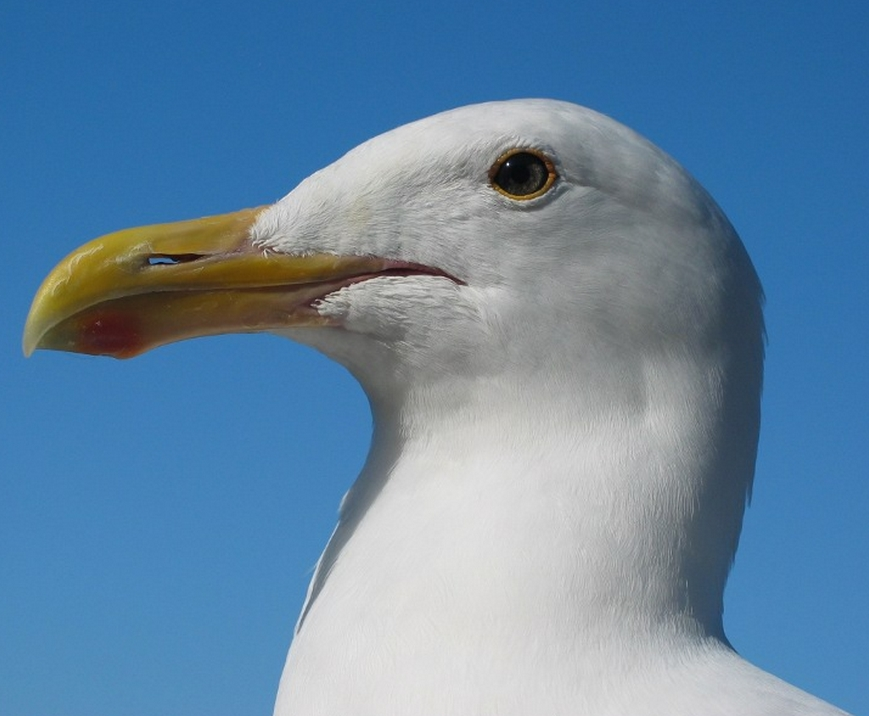
\includegraphics[width=0.75\textwidth,]{Figures_Chapter_1/bird.jpg}
	\caption{Bird in JPEG format}
	\label{bird_jpeg}
\end{figure}

The PDF format can also be used in Figure \ref{bird_pdf}

\begin{figure}[!h]
	\centering
	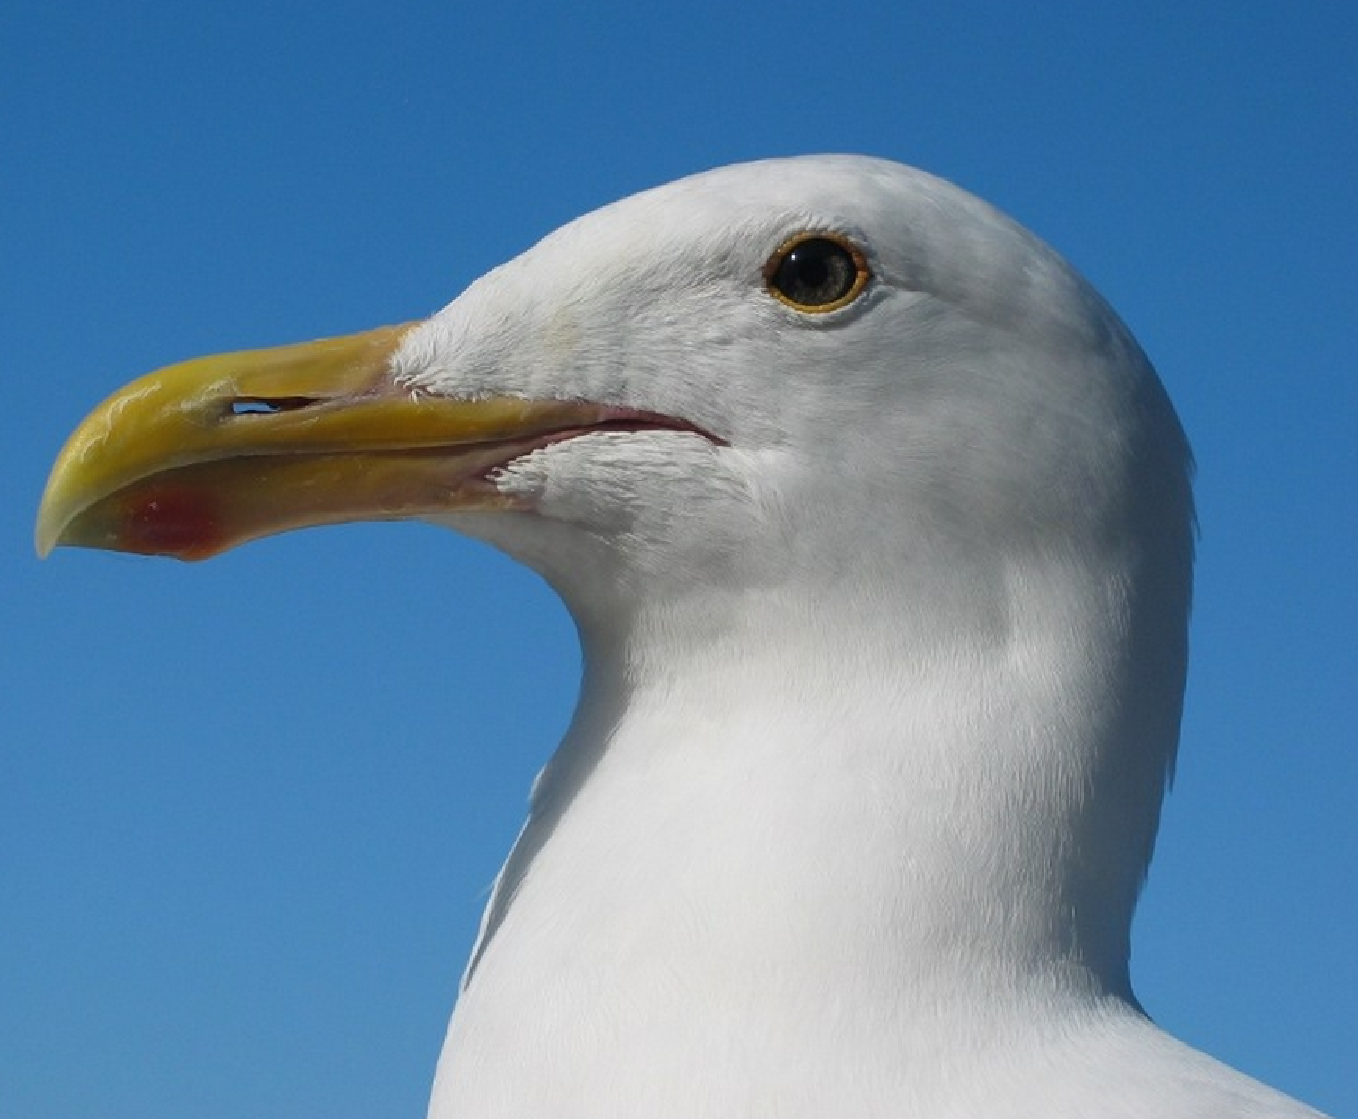
\includegraphics[width=0.75\textwidth,]{Figures_Chapter_1/bird.pdf}
	\caption{Bird in JPEG format}
	\label{bird_pdf}
\end{figure}

\section{Conclusion}

This chapter has provided an overview of the X ...

The main contributions of these dissertations are thoroughly presented in the following chapters.
	
	\chapter{Title of Chapter 2}

\section{Introduction}

Text of introduction

\section{Section}

For complex equations, we can define an example of mathematical equation in \eqref{MDDRV}:
\begin{equation}
	\label{MDDRV}
	\begin{split}
		y(n)=&\sum_{k=0}^{\frac{K-1}{2}}\sum_{i=0}^{M}a_{2k+1,1}|x(n)|^{2k}x(n-i)\\
		&+\sum_{k=1}^{\frac{K-1}{2}}\sum_{i=1}^{M}a_{2k+1,2}|x(n)|^{2(k-1)}x^2(n)x^*(n-i)\\
		&+\sum_{k=1}^{\frac{K-1}{2}}\sum_{i=1}^{M}a_{2k+1,3}|x(n)|^{2(k-1)}x(n)|x(n-i)|^2\\
		&+\sum_{k=1}^{\frac{K-1}{2}}\sum_{i=1}^{M}a_{2k+1,4}|x(n)|^{2(k-1)}x^*(n)x^2(n-i)\\
		&+\sum_{k=1}^{\frac{K-1}{2}}\sum_{i=1}^{M}b_{2k+1}|x(n-i)|^{2k}x(n-i)
	\end{split}
\end{equation}

The matrix of a given model can be represented as:
\begin{equation}
	\small
	\textbf{Z}=\left[
	\begin{array}{llllll}
		\Phi_{1,1}(z(n)) & \dots & \Phi_{K,1}(z(n)) & \Phi_{1,2}(z(n)) & \cdots & \Phi_{K,L}(z(n)) \\
		\Phi_{1,1}(z(n-1)) & \vdots & \ddots &  & \vdots & \Phi_{K,L}(z(n-1)) \\
		\vdots & \vdots &  &  &  & \vdots \\
		\Phi_{1,1}(z(n-N+1)) & \cdots &  &  &  & \Phi_{K,L}(z(n-N+1)) \\ %z(n-N-L+2)|z(n-N-L+2)|^{K-1}
	\end{array}
	\right]
\end{equation}
where $\Phi_{k,l}(z(n))=z(n-l+1)|z(n-l+1)|^{k-1}$.

Table \ref{TabTest1} presents an example of tables

\newpage

\begin{table}[!h]
	\centering
	\caption{Comparison}
	%\begin{adjustbox}{width=\columnwidth,center}
	\begin{tabular}{|c|c|c|}
		\hline
		\textbf{Model } & \multirow{2}{*}{\textbf{Parameters}} & \textbf{Number} \\
		\textbf{for Comparison} &  & \textbf{of parameters} \\
		\hline
		\hline
		\multirow{2}{*}{Model 1} & $A$: parameter 1 & \multirow{2}{*}{$ A+B $}\\
		& $B$: parameter 2 & \\
		\hline
		\multirow{2}{*}{Model 2} & $A$: parameter 1 & \multirow{2}{*}{$A+B$}\\
		& $B$: parameter 2 & \\
		\hline
	\end{tabular}
	\label{TabTest1}
	%\end{adjustbox}
\end{table}

For large tables, you have to use the package \textit{adjustbox} to re-size the table according to the width of the document.	

\section{Conclusion}

This chapter introduces the principle of ...

For that purpose, the following chapter will focus on ...

	\chapter{Optimization and Sizing of DVR Model} 

\section{Introduction}

Text of introduction ...

\section{Section 1}

An example of Algorithm of a given mathematical behavior of $f(x_1)$ and $f(x_2)$ is illustrated in Algorithm \eqref{Algo}.

\begin{algorithm}[!h]
	\caption{Algorithm of test}
	$q=0$ ; $a_0=a$ ; $b_0=b$ \\
	Compute $x_1$ and $x_2$ \\
	\While{$|b_q-a_q|>\epsilon$}{
		Compute $f(x_1)$ and $f(x_2)$ \\
		\If{$f(x_1)\leq f(x_2)$}{
			$a_{q+1}=a_q$ \\
			$b_{q+1}=x_2$ \\
			$x_2=x_1$ \\
			Compute $x_1$  \\
		}
		$q=q+1$
	}
	$x_{opt}=\frac{a_{q}+b_{q}}{2}$
	\label{Algo}
\end{algorithm}

Table \ref{TabTest2} present an example of complex tables.

\newpage

\begin{table*}[!h]
	\centering
	\caption{Comparison of criterion 1, 2, and 3}
	%\begin{adjustbox}{width=\columnwidth,center}
		\begin{tabular}{|c|c|c|c|c|}
			\cline{3-5}
			\multicolumn{2}{c|}{}  & Uniform & \multicolumn{2}{|c|}{Random} \\
			\multicolumn{2}{c|}{}  & Test &  \multicolumn{2}{|c|}{Test} \\
			\cline{4-5}
			\multicolumn{2}{c|}{}  & & Best case & Worst case \\
			\hline
			\multicolumn{2}{|c|}{Results} & \multirow{2}{*}{$[1.11~2.22~3.33]$}  & \multirow{2}{*}{$[1.11~2.22~3.33]$} & \multirow{2}{*}{$[1.11~2.22~3.33]$} \\
			\multicolumn{2}{|c|}{before optimization} &  &  & \\
			\hline
			\multicolumn{2}{|c|}{Index 1} & 14.98 & 38.68 & 12.09 \\
			\hline
			\multicolumn{5}{|c|}{\textbf{Application of our approach}}  \\
			\hline
			\multicolumn{2}{|c|}{Optimization of} & \multirow{2}{*}{$[1.11~2.22~3.33]$} & \multirow{2}{*}{$[1.11~2.22~3.33]$} & \multirow{2}{*}{$[1.11~2.22~3.33]$}\\
			\multicolumn{2}{|c|}{Results} & & & \\
			\hline
			\multicolumn{2}{|c|}{Index 1}  & 20.76 & 45.09 & 23.98 \\
			\hline
			\cline{2-5}
			\multicolumn{1}{|c|}{\multirow{2}{*}{Index 2} }& Left & 18.49 & 18.49 & 18.49\\
			\cline{2-5}
			& Right & 18.82 & 19.82 & 19.82\\
			\cline{2-5}
			\hline
			\multicolumn{1}{|c|}{\multirow{3}{*}{Index 3} } & Left & 4 & 1 & 2 \\
			\cline{2-5}
			& Center & 2 & 3 & 5 \\
			\cline{2-5}
			& Right & 3 & 1 & 2\\
			\hline
		\end{tabular}
		\label{TabTest2}
	%\end{adjustbox}
\end{table*}

\section{Section 2} % \label{SectionHC} % You can add a label to reference this section

\subsection{Sub-Section 1}

\subsubsection{Sub Sub-Section 1}

\paragraph{Paragraph} \mbox{}\\

\subparagraph{Sub-Paragraph} \mbox{}\\

You can enumerate the sub paragraph by changing the number in used to set counter in \textit{setcounter\{secnumdepth\}\{5\}}


\section{Conclusion}

In this chapter, X are discussed and investigated ...
	
	\addcontentsline{toc}{chapter}{Conclusion and Perspectives}
	
	\chapter*{Conclusion and Perspectives}
	
	\section*{Contributions}
	
	In this dissertation, we have focused on ...
	This dissertation mainly focuses on three aspects ...
	
	\begin{enumerate}
		\item Aspect 1.
		
		\item Aspect 2.
		
		\item Aspect 3 ...
	\end{enumerate}
	
	\section*{Perspectives}
	
	To extend this dissertation, some research works could be developed:
	
	\begin{enumerate}
		\item Perspective 1.
		
		\item Perspective 2.
		
		\item Perspective 3 ...		
	\end{enumerate}
	
	Further research works are currently in progress for submission, which are listed along with the abstract:
	
	\begin{itemize}
		\item Author 1, Author 2 and Author 3, “Title of paper 1”.
		
		$-$ Abstract: \textit{Abstract of paper}
		
		\item Author 1, Author 2 and Author 3, “Title of paper 2”.
		
		$-$ Abstract: \textit{Abstract of paper2}
		
		\item Author 1, Author 2 and Author 3, “Title of paper 3”.
		
		$-$ Abstract: \textit{Abstract of paper 3}
		 
	\end{itemize}
	
	\chapter*{Résumé détaillé de la thèse en français \\ $~$ \\ \Large \textit{Titre de thèse}}

\addcontentsline{toc}{chapter}{Résumé détaillé de la thèse en français}

Introduction

\section*{Cnntribution 1}

Texte de la contribution 1.

\section*{Cnntribution 2}

Texte de la contribution 2.

\section*{Cnntribution 3}

Texte de la contribution 3 ...

\section*{Conclusion et perspectives}

Dans cette thèse, nous nous sommes concentrés sur ...

\begin{enumerate}
	\item Contribution 1.
	
	\item Contribution 2.
	
	\item Contribution 3 ...
\end{enumerate}
	
	
	\newpage
	
	$~$
	
	\newpage
	
	\addcontentsline{toc}{chapter}{Bibliography}
	
	\begin{thebibliography}{biblio}
	%chapitre 1
	\bibitem{Author2020} Author 1. Author 2, Author 3, "Title of paper," in IEEE Microwave Magazine, vol. 11, no. 5, pp. 44-58, Aug. 2020.	
\end{thebibliography}

	
	\newpage
	
	\thispagestyle{empty}
	
	\mbox{}
	
	\newpage
	
	\newpage
	
	\section*{Abstract}
	
	Abstract of Ph.D. in english
	
	\section*{R\'esum\'e}
	
	Resume de la these en francais
	
\end{document}          
